\section{Mathematical Formulation}\label{sec:formulation}

\subsection{Model Geometry and Assumptions}\label{sec:geometry}

The human abdominal cavity is idealised as an oblate spheroidal shell of
semi-major axes $a$ (equatorial, in the lateral and cranio-caudal directions)
and semi-minor axis $c$ (antero-posterior), with $c < a$.  The shell has uniform
wall thickness $h$ and is completely filled with an inviscid, irrotational
fluid of density $\rho_f$ and bulk modulus $K_f$.  Following standard practice
in fluid-filled shell analysis \cite{Junger1986,lamb1882} and recent
experimental and analytical studies of pressurised elastic shells
\cite{Kuo2015,Ghaheri2022}, an
equivalent-sphere radius is defined via
\begin{equation}\label{eq:Req}
  R_\mathrm{eq} = (a^2 c)^{1/3},
\end{equation}
which preserves the cavity volume, $V = \tfrac{4}{3}\pi a^2 c$.  This
approximation is exact for a sphere ($c = a$) and introduces errors of order
$(1 - c/a)^2$ for the eigenfrequencies at moderate aspect ratios ($c/a \gtrsim
0.5$).  Table~\ref{tab:params} lists the baseline geometric and material
parameters with physiological justification.

The thin-shell assumption ($h/R_\mathrm{eq} \ll 1$) is satisfied: for
$h = 10$\,mm and $R_\mathrm{eq} \approx 157$\,mm, $h/R \approx 0.06$.  The
Love--Kirchhoff hypothesis (normals remain straight and normal to the
deformed mid-surface) is therefore applicable.  This linear framework remains
the standard starting point even in modern reviews of nonlinear shell
vibration, which treat geometric nonlinearities as amplitude corrections to
the same modal backbone \cite{Alijani2014}.

\begin{table}[htbp]
  \centering
  \caption{Baseline model parameters with physiological justification.}
  \label{tab:params}
  \begin{tabular}{lcccl}
    \hline
    Parameter & Symbol & Value & Unit & Source \\
    \hline
    Semi-major axis & $a$ & 0.18 & m & Anthropometric mean \\
    Semi-minor axis & $c$ & 0.12 & m & $c/a \approx 0.67$ \\
    Wall thickness & $h$ & 0.010 & m & Composite wall \\
    Elastic modulus & $E$ & 0.1 & MPa & Representative of reported measurements \cite{Deeken2017} \\
    Poisson's ratio & $\nu$ & 0.45 & --- & Near-incompressible modelling convention \cite{Spadoni2024} \\
    Wall density & $\rho_w$ & 1100 & kg/m$^3$ & Soft tissue \\
    Fluid density & $\rho_f$ & 1020 & kg/m$^3$ & Abdominal fluid \\
    Fluid bulk modulus & $K_f$ & 2.2 & GPa & Water at 37$^\circ$C \\
    Intra-abdominal pressure & $P_\mathrm{iap}$ & 1000 & Pa & Representative resting clinical measurement \cite{Novak2021} \\
    Loss tangent & $\eta$ & 0.25 & --- & Representative review value \cite{Sack2023} \\
    \hline
  \end{tabular}
\end{table}

\begin{figure}[htbp]
  \centering
  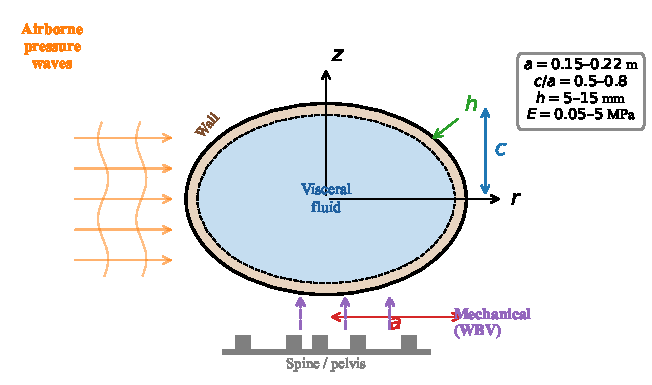
\includegraphics[width=\textwidth]{../data/figures/fig_geometry_schematic.pdf}
  \caption{Oblate spheroidal shell model of the human abdominal cavity,
  showing the two excitation pathways: airborne acoustic pressure (left)
  and mechanical whole-body vibration transmitted through the skeleton (right).
  Dimensions correspond to the baseline parameters in Table~\ref{tab:params}.}
  \label{fig:geometry}
\end{figure}

Figure~\ref{fig:geometry} illustrates the model geometry and the two excitation
pathways.  The abdominal wall is modelled as a Kelvin--Voigt viscoelastic material with
complex modulus
\begin{equation}\label{eq:Estar}
  E^* = E(1 + i\eta),
\end{equation}
where $\eta$ is the loss tangent.  For small damping, the quality factor is
$Q = 1/\eta$ and the viscous damping ratio is $\zeta = \eta/2 = 1/(2Q)$.  The
flexural rigidity of the shell is
\begin{equation}\label{eq:D}
  D = \frac{Eh^3}{12(1 - \nu^2)}.
\end{equation}
These baseline values are not arbitrary.  The canonical modulus
$E = \SI{0.1}{\mega\pascal}$ is representative of direct abdominal-wall
measurements compiled by Deeken and Lake \cite{Deeken2017};
$\nu = 0.45$ follows the nearly incompressible modelling convention adopted in
recent abdominal-wall finite-element studies \cite{Spadoni2024}; resting
intra-abdominal pressures of 5--12\,mmHg correspond to approximately
\SIrange{0.67}{1.60}{\kilo\pascal}, so
$P_\mathrm{iap} = \SI{1.0}{\kilo\pascal}$ is representative of direct clinical
measurements \cite{Novak2021}; and modern elastography reviews place the
soft-tissue loss tangent broadly in the 0.1--0.4 range, making
$\eta = 0.25$ consistent with the range reported for soft tissue
\cite{Sack2023}.  Published values of $\eta$ for abdominal
soft tissue range from 0.15 to 0.40 at low frequencies
\cite{parker2011imaging}, corresponding to $Q = 2.5$--$6.7$.  The baseline
value $\eta = 0.25$ ($Q = 4.0$, $\zeta = 0.125$) represents a central estimate.


\subsection{Breathing Mode (\texorpdfstring{$n = 0$}{n = 0})}\label{sec:breathing}

The breathing mode is a spatially uniform radial oscillation in which the shell
displaces by $\xi$ at every point.  The associated volumetric strain is
$\Delta V/V = 3\xi/R$, which compresses the contained fluid.  Two restoring
forces act on the shell:

\paragraph{Membrane stiffness.}
For the uniform expansion of a thin spherical shell,
\begin{equation}\label{eq:kshell}
  k_\mathrm{shell} = \frac{2Eh}{R^2(1 - \nu)}.
\end{equation}

\paragraph{Fluid volumetric stiffness.}
The pressure increment due to fluid compression is $\Delta p = K_f \Delta V /
V = 3K_f \xi / R$.  The restoring force per unit displacement per unit area is
\begin{equation}\label{eq:kfluid}
  k_\mathrm{fluid} = \frac{3K_f}{R}.
\end{equation}
With $K_f = 2.2$\,GPa and $R = 0.157$\,m, $k_\mathrm{fluid} = 4.2 \times
10^{10}$\,Pa/m, which exceeds the membrane stiffness ($k_\mathrm{shell}
\approx 1.5 \times 10^5$\,Pa/m) by five orders of magnitude.  \emph{The
breathing mode is entirely dominated by the fluid bulk modulus.}

The effective mass per unit area includes the shell wall and the fluid added
mass for the $n = 0$ mode:
\begin{equation}\label{eq:m0}
  m_\mathrm{eff}^{(0)} = \rho_w h + \rho_f R.
\end{equation}

The breathing mode frequency is therefore
\begin{equation}\label{eq:f0}
  f_0 = \frac{1}{2\pi}\sqrt{\frac{k_\mathrm{shell} + k_\mathrm{fluid}}
  {\rho_w h + \rho_f R}} \approx 2500\;\text{Hz},
\end{equation}
which lies in the kilohertz range and is irrelevant to infrasonic exposure.
This result is robust to material property variations because $k_\mathrm{fluid}
\gg k_\mathrm{shell}$ for any realistic shell stiffness.


\subsection{Flexural Modes (\texorpdfstring{$n \geq 2$}{n >= 2})}\label{sec:flexural}

Flexural modes involve shape changes (oblate--prolate oscillation for $n = 2$,
trilobed for $n = 3$, etc.)\ that preserve the enclosed volume to leading
order.  The fluid therefore does \emph{not} act as a volumetric spring; it
contributes only added mass.

Following Lamb \cite{lamb1882} and Junger \& Feit
\cite{Junger1986}, with subsequent validation in modern pressurised-shell
studies \cite{Kuo2015,Ghaheri2022}, the flexural mode of order $n$ has three contributions
to the restoring force per unit area.  (An analogous modal decomposition
for fluid-filled elastic tubes in biological contexts was developed by
Heil~\cite{Heil1996}.)

\paragraph{Bending stiffness.}
\begin{equation}\label{eq:Kbend}
  K_\mathrm{bend} = \frac{n(n-1)(n+2)^2 D}{R^4}.
\end{equation}

\paragraph{Membrane stiffness.}
\begin{equation}\label{eq:Kmemb}
  K_\mathrm{memb} = \frac{Eh}{R^2}\,\lambda_n,
  \qquad \lambda_n = \frac{n^2 + n - 2 + 2\nu}{n^2 + n + 1 - \nu}.
\end{equation}

\paragraph{Pre-stress stiffness.}
The static intra-abdominal pressure $P$ produces a pre-stress in the
shell membrane that stiffens flexural modes:
\begin{equation}\label{eq:Kpre}
  K_P = \frac{P}{R}(n-1)(n+2).
\end{equation}

The fluid added mass per unit area for mode $n$ is
\begin{equation}\label{eq:madd}
  m_\mathrm{add}^{(n)} = \frac{\rho_f R}{n},
\end{equation}
giving a total effective mass of
\begin{equation}\label{eq:meff}
  m_\mathrm{eff}^{(n)} = \rho_w h + \frac{\rho_f R}{n}.
\end{equation}

The natural frequency of flexural mode $n$ is
\begin{equation}\label{eq:fn}
  \omega_n^2 = \frac{K_\mathrm{bend} + K_\mathrm{memb} + K_P}
                    {m_\mathrm{eff}^{(n)}},
  \qquad f_n = \frac{\omega_n}{2\pi}.
\end{equation}

For the baseline parameters (Table~\ref{tab:params}), $f_2 = 4.0$\,Hz,
$f_3 = 6.3$\,Hz, and $f_4 = 8.9$\,Hz (Figure~\ref{fig:modes}).  (The $n = 1$
mode corresponds to rigid-body translation and has zero natural frequency for
a free shell; it is therefore excluded.)  These lie squarely in the 4--10\,Hz
range reported for abdominal resonance in ISO~2631 \cite{iso2631} and in the
experimental studies of Kitazaki \& Griffin \cite{kitazaki1998resonance} and
Mansfield \cite{mansfield2005human}.

\begin{figure}[htbp]
  \centering
  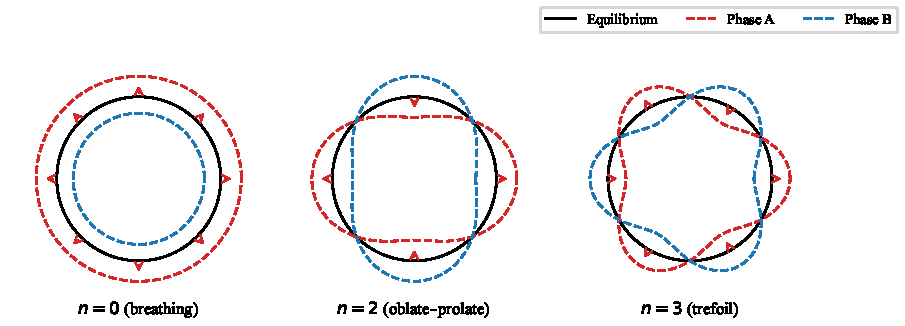
\includegraphics[width=\textwidth]{../data/figures/fig_mode_shapes.pdf}
  \caption{Schematic cross-sections of the first three mode families.
  The breathing mode ($n=0$) involves uniform radial expansion against
  the fluid bulk modulus.  Flexural modes ($n=2, 3$) deform the shell
  shape without significant volume change; the enclosed fluid acts as
  added mass only.}
  \label{fig:modes}
\end{figure}


\subsection{Airborne Acoustic Coupling}\label{sec:airborne}

We now quantify the excitation of flexural modes by an incident airborne
acoustic field.  At $f_2 \approx 4$\,Hz, the acoustic wavelength in air is
$\lambda \approx 87$\,m, so the dimensionless wavenumber is
\begin{equation}\label{eq:ka}
  ka = \frac{2\pi f_2 R_\mathrm{eq}}{c_\mathrm{air}} \approx 0.0114 \ll 1.
\end{equation}
The body is deep in the sub-wavelength (Rayleigh scattering) regime.

In a multipole expansion of the incident plane wave scattered by a sphere, the
$n$-th order component of the pressure field scales, to leading order, as
\cite{Junger1986}:
\begin{equation}\label{eq:peff}
  p_\mathrm{eff}^{(n)} \propto p_\mathrm{inc} (ka)^n.
\end{equation}
The breathing mode ($n = 0$) sees the full incident pressure, but flexural
modes ($n \geq 2$) see only the higher-order spatial gradients, which are
vanishingly small when $ka \ll 1$.  For $n = 2$:
\begin{equation}\label{eq:peff2}
  p_\mathrm{eff}^{(2)} = p_\mathrm{inc} \times (ka)^2
  \approx p_\mathrm{inc} \times 1.3 \times 10^{-4}.
\end{equation}

The displacement at resonance ($\omega = \omega_n$) is
\begin{equation}\label{eq:xi_air}
  \xi_\mathrm{air} = \frac{p_\mathrm{eff}^{(n)}}{K_\mathrm{total}^{(n)}} Q,
\end{equation}
where $K_\mathrm{total}^{(n)} = K_\mathrm{bend} + K_\mathrm{memb} + K_P$.
At 120\,dB SPL ($p_\mathrm{inc} = 20$\,Pa), the energy-consistent reciprocity
analysis (\S\ref{sec:coupling}) gives
$\xi_\mathrm{air} \approx 0.014$\,$\mu$m for $n = 2$ --- well below the
0.5--2.0\,$\mu$m activation threshold of mechanosensitive ion channels
\cite{coste2010piezo1}.  (The pressure-based estimate of
equation~\eqref{eq:xi_air} yields $\approx 0.18$\,$\mu$m, an overestimate
that violates the energy budget; see \S\ref{sec:coupling}.)


\subsection{Mechanical (Whole-Body Vibration) Coupling}\label{sec:wbv}

Whole-body vibration (WBV) transmits through the skeleton and acts as
\emph{base excitation} of the abdominal shell.  Unlike airborne acoustic
coupling, there is no impedance mismatch and no $(ka)^n$ penalty.  The
vibration is transmitted at full amplitude through the rigid skeletal frame.

For harmonic base acceleration $a_\mathrm{base}(t) = a_0 \cos(\omega t)$, the
base displacement amplitude is
\begin{equation}\label{eq:xbase}
  x_\mathrm{base} = \frac{a_\mathrm{rms} \sqrt{2}}{\omega^2}.
\end{equation}

The relative displacement between the shell and the skeleton is given by the
base-excitation frequency response function:
\begin{equation}\label{eq:Hrel}
  H_\mathrm{rel}(\omega) = \frac{r^2}{\sqrt{(1-r^2)^2 + (2\zeta r)^2}},
  \qquad r = \frac{\omega}{\omega_n},
\end{equation}
so that
\begin{equation}\label{eq:xi_mech}
  \xi_\mathrm{mech} = x_\mathrm{base} \times H_\mathrm{rel}.
\end{equation}

At the EU Whole-Body Vibration Directive exposure limit of
$a_\mathrm{rms} = 1.15$\,m/s$^2$ and at the $n = 2$ resonance frequency:
\begin{equation}
  \xi_\mathrm{mech} \approx 10{,}500\;\mu\text{m} \approx 10\;\text{mm},
\end{equation}
which exceeds the mechanotransduction threshold by more than three orders
of magnitude.


\subsection{Coupling Ratio}\label{sec:ratio}

The ratio of mechanical to airborne displacement at the same excitation
conditions provides a dimensionless measure of the full coupling disparity:
\begin{equation}\label{eq:coupling_ratio_def}
  \mathcal{R}_\mathrm{full} = \frac{\xi_\mathrm{mech}}{\xi_\mathrm{air}}.
\end{equation}

This ratio depends primarily on $ka$ and the excitation level, and is
\emph{robust} to uncertainties in material properties and boundary conditions
because both pathways excite the same modal structure.  The full coupling ratio
is the central result of this work: it provides a quantitative explanation for why
whole-body vibration at 4--8\,Hz is associated with gastrointestinal effects in
the epidemiological literature \cite{griffin1990handbook}, whereas airborne
infrasound at comparable frequencies is not.  Section~\ref{sec:coupling}
shows that, for \SI{120}{\decibel} SPL airborne excitation and
$a_\mathrm{rms} = \SI{0.1}{\metre\per\second\squared}$ RMS whole-body
vibration, the SDOF upper bound is $\mathcal{R}_\mathrm{full} \approx 6.6 \times 10^4$
($\Gamma_2 = 1$), reducing to $\sim 3 \times 10^4$ when the canonical
participation factor $\Gamma_2 \approx 0.48$ is included.
